\PassOptionsToPackage{unicode=true}{hyperref} % options for packages loaded elsewhere
\PassOptionsToPackage{hyphens}{url}
%
\documentclass[ignorenonframetext,]{beamer}
\usepackage{pgfpages}
\setbeamertemplate{caption}[numbered]
\setbeamertemplate{caption label separator}{: }
\setbeamercolor{caption name}{fg=normal text.fg}
\beamertemplatenavigationsymbolsempty
\usepackage{lmodern}
\usepackage{amssymb,amsmath}
\usepackage{ifxetex,ifluatex}
\usepackage{fixltx2e} % provides \textsubscript
\ifnum 0\ifxetex 1\fi\ifluatex 1\fi=0 % if pdftex
  \usepackage[T1]{fontenc}
  \usepackage[utf8]{inputenc}
  \usepackage{textcomp} % provides euro and other symbols
\else % if luatex or xelatex
  \usepackage{unicode-math}
  \defaultfontfeatures{Ligatures=TeX,Scale=MatchLowercase}
\fi
% use upquote if available, for straight quotes in verbatim environments
\IfFileExists{upquote.sty}{\usepackage{upquote}}{}
% use microtype if available
\IfFileExists{microtype.sty}{%
\usepackage[]{microtype}
\UseMicrotypeSet[protrusion]{basicmath} % disable protrusion for tt fonts
}{}
\IfFileExists{parskip.sty}{%
\usepackage{parskip}
}{% else
\setlength{\parindent}{0pt}
\setlength{\parskip}{6pt plus 2pt minus 1pt}
}
\usepackage{hyperref}
\hypersetup{
            pdftitle={An introduction to GAM(M)s},
            pdfauthor={Stefano Coretta},
            pdfborder={0 0 0},
            breaklinks=true}
\urlstyle{same}  % don't use monospace font for urls
\newif\ifbibliography
\usepackage{graphicx,grffile}
\makeatletter
\def\maxwidth{\ifdim\Gin@nat@width>\linewidth\linewidth\else\Gin@nat@width\fi}
\def\maxheight{\ifdim\Gin@nat@height>\textheight\textheight\else\Gin@nat@height\fi}
\makeatother
% Scale images if necessary, so that they will not overflow the page
% margins by default, and it is still possible to overwrite the defaults
% using explicit options in \includegraphics[width, height, ...]{}
\setkeys{Gin}{width=\maxwidth,height=\maxheight,keepaspectratio}
% Prevent slide breaks in the middle of a paragraph:
\widowpenalties 1 10000
\raggedbottom
\setbeamertemplate{part page}{
\centering
\begin{beamercolorbox}[sep=16pt,center]{part title}
  \usebeamerfont{part title}\insertpart\par
\end{beamercolorbox}
}
\setbeamertemplate{section page}{
\centering
\begin{beamercolorbox}[sep=12pt,center]{part title}
  \usebeamerfont{section title}\insertsection\par
\end{beamercolorbox}
}
\setbeamertemplate{subsection page}{
\centering
\begin{beamercolorbox}[sep=8pt,center]{part title}
  \usebeamerfont{subsection title}\insertsubsection\par
\end{beamercolorbox}
}
\AtBeginPart{
  \frame{\partpage}
}
\AtBeginSection{
  \ifbibliography
  \else
    \frame{\sectionpage}
  \fi
}
\AtBeginSubsection{
  \frame{\subsectionpage}
}
\setlength{\emergencystretch}{3em}  % prevent overfull lines
\providecommand{\tightlist}{%
  \setlength{\itemsep}{0pt}\setlength{\parskip}{0pt}}
\setcounter{secnumdepth}{0}

% set default figure placement to htbp
\makeatletter
\def\fps@figure{htbp}
\makeatother

\setbeamertemplate{navigation symbols}{}
\setbeamertemplate{footline}[page number]
\linespread{1.5}

\title{An introduction to GAM(M)s}
\author{Stefano Coretta}
\date{12/07/2018}

\begin{document}
\frame{\titlepage}

\begin{frame}{Linear models}
\protect\hypertarget{linear-models}{}

\centering \Huge

Time travel\ldots{}

\end{frame}

\begin{frame}{Linear models}
\protect\hypertarget{linear-models-1}{}

\centering \Huge

\(y = 3 + 2x\)

\large

where \(x = (2, 4, 5, 8, 10, 23, 36)\)

\end{frame}

\begin{frame}{Linear models}
\protect\hypertarget{linear-models-2}{}

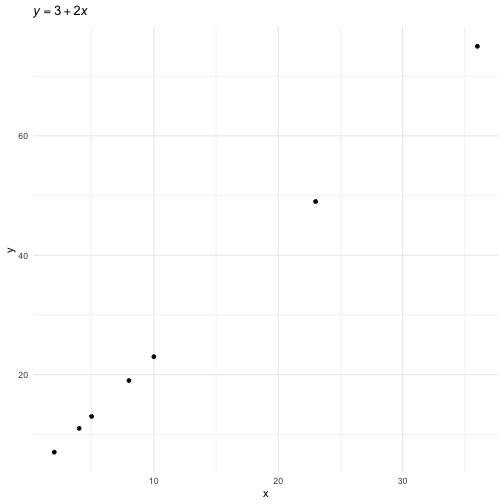
\includegraphics{gamm-presentation_files/figure-beamer/homework-1.pdf}

\end{frame}

\begin{frame}{Linear models}
\protect\hypertarget{linear-models-3}{}

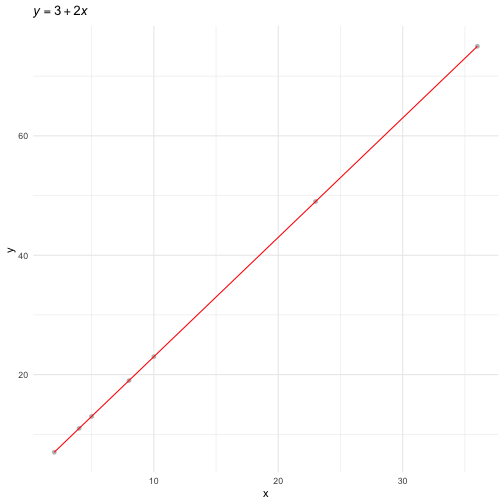
\includegraphics{gamm-presentation_files/figure-beamer/line-1.pdf}

\end{frame}

\begin{frame}{Linear models}
\protect\hypertarget{linear-models-4}{}

\begin{itemize}
\item
  In science, we have \(x\) and \(y\)\ldots{}
\item
  for example, vowel duration and VOT
\end{itemize}

\end{frame}

\begin{frame}{Linear models}
\protect\hypertarget{linear-models-5}{}

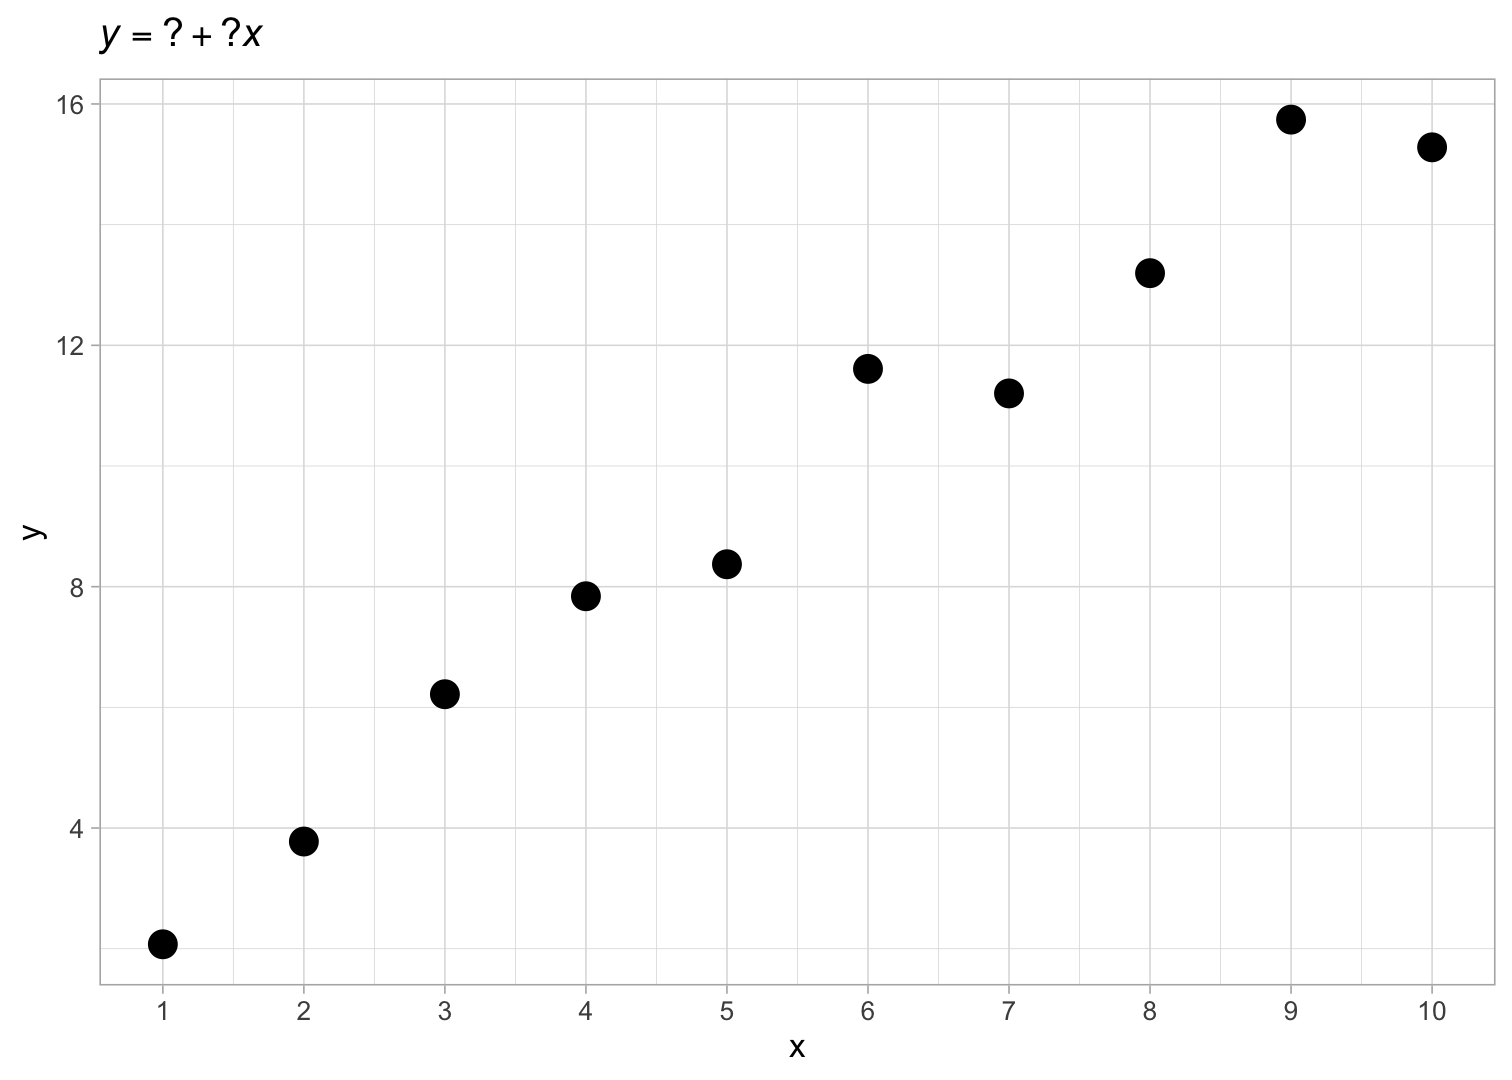
\includegraphics{gamm-presentation_files/figure-beamer/sampled-1.pdf}

\end{frame}

\begin{frame}[fragile]{Linear models}
\protect\hypertarget{linear-models-6}{}

\begin{itemize}
\tightlist
\item
  The formula: \(y = \beta_0 + \beta_1x\)

  \begin{itemize}
  \tightlist
  \item
    \(\beta_0\) is the \textbf{intercept}
  \item
    \(\beta_1\) is the \textbf{slope}
  \end{itemize}
\item
  We know \(x\) and \(y\)

  \begin{itemize}
  \tightlist
  \item
    we need to estimate \(\beta_0\), \(\beta_1\) =
    \(\hat{\beta_0}, \hat{\beta_1}\)
  \end{itemize}
\item
  We can add more predictors

  \begin{itemize}
  \tightlist
  \item
    \(y = \beta_0 + \beta_1x_1 + \beta_2x_2 + ... + \beta_nx_n\)
  \end{itemize}
\item
  \texttt{lm(y\ \textasciitilde{}\ x,\ data)} (`\(y\) as a function of
  \(x\)')
\end{itemize}

\end{frame}

\begin{frame}{Linear models}
\protect\hypertarget{linear-models-7}{}

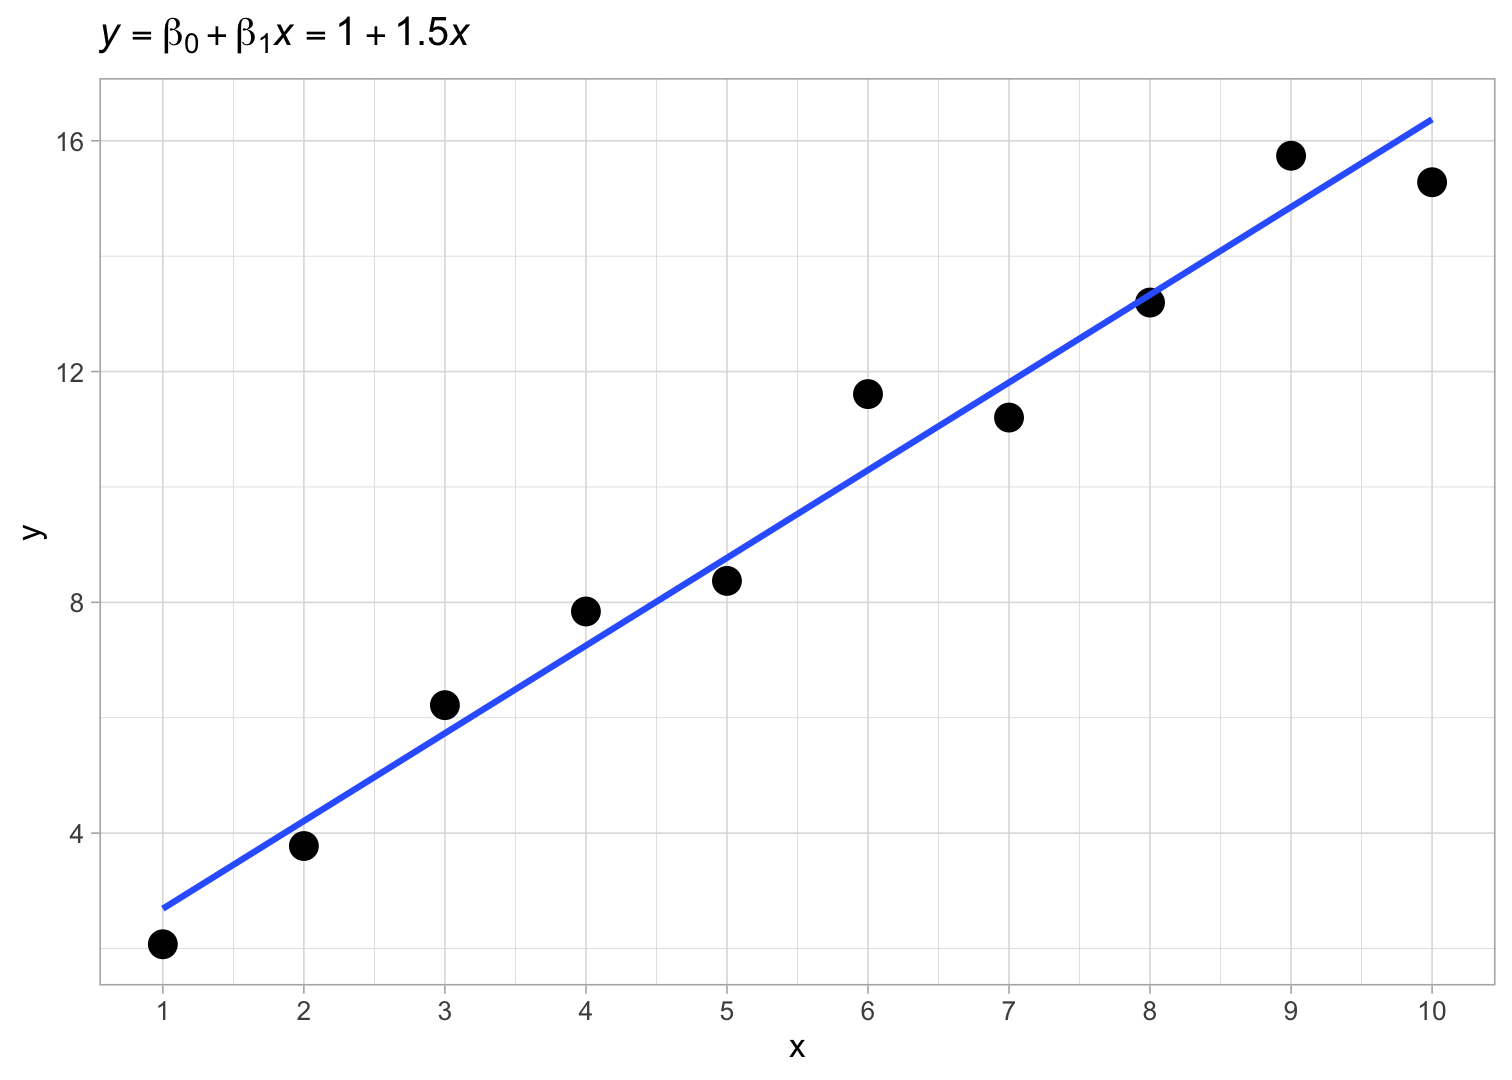
\includegraphics{gamm-presentation_files/figure-beamer/lm-plot-1.pdf}

\end{frame}

\begin{frame}{Linear models}
\protect\hypertarget{linear-models-8}{}

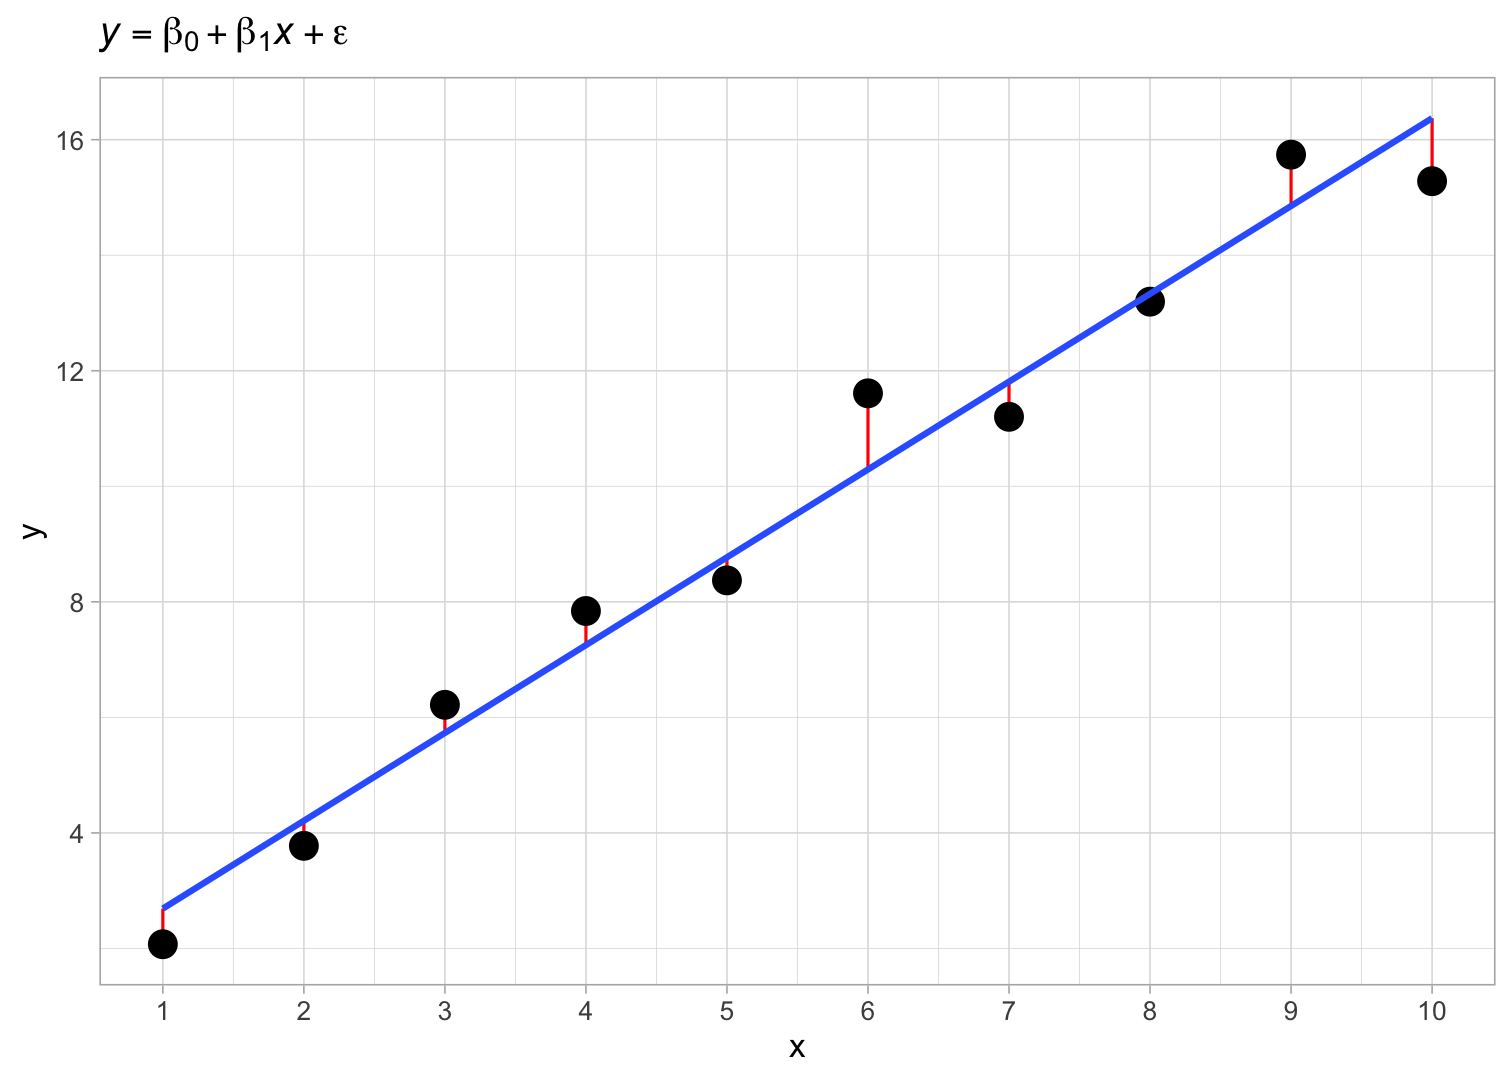
\includegraphics{gamm-presentation_files/figure-beamer/error-1.pdf}

\end{frame}

\begin{frame}{LM with non-linear data}
\protect\hypertarget{lm-with-non-linear-data}{}

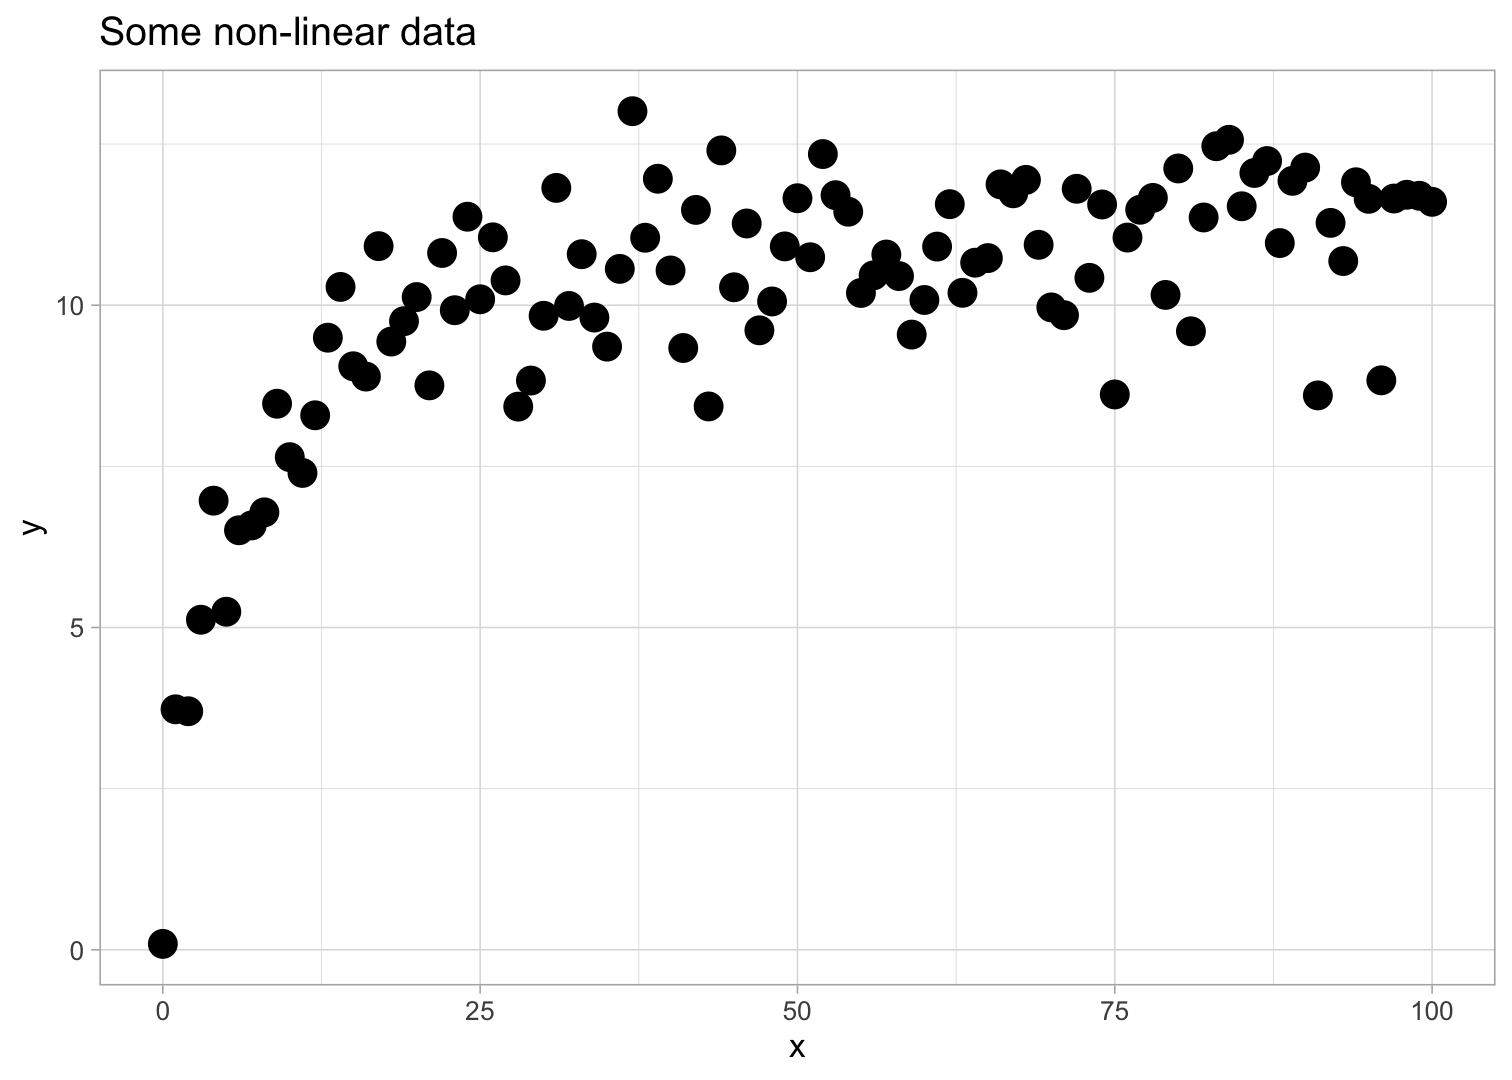
\includegraphics{gamm-presentation_files/figure-beamer/plot-data-1.pdf}

\end{frame}

\begin{frame}{LM with non-linear data}
\protect\hypertarget{lm-with-non-linear-data-1}{}

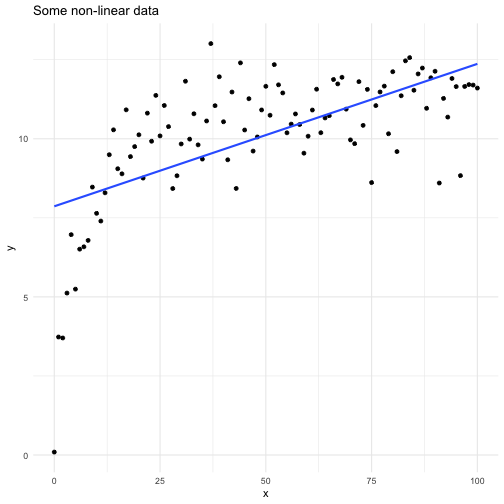
\includegraphics{gamm-presentation_files/figure-beamer/plot-lm-1.pdf}

\end{frame}

\begin{frame}{LM with non-linear data}
\protect\hypertarget{lm-with-non-linear-data-2}{}

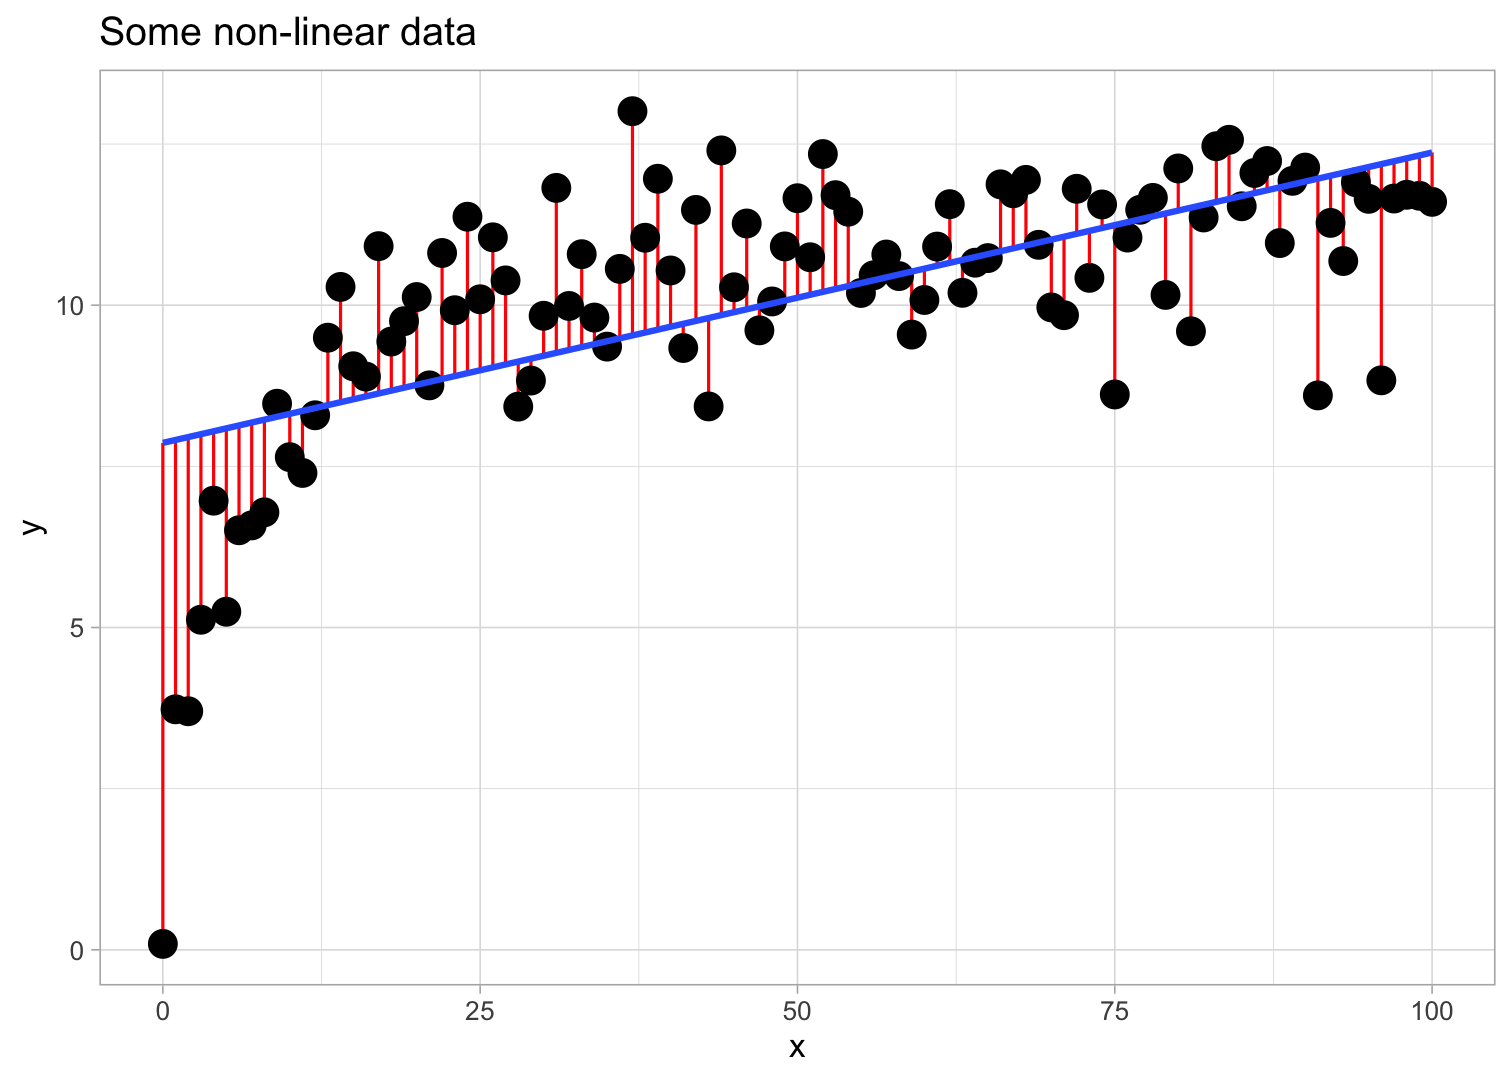
\includegraphics{gamm-presentation_files/figure-beamer/error-2-1.pdf}

\end{frame}

\begin{frame}{LM with non-linear data}
\protect\hypertarget{lm-with-non-linear-data-3}{}

How to account for non-linearity in a linear model?

\begin{itemize}
\tightlist
\item
  Use \textbf{higher-degree polynomials}

  \begin{itemize}
  \tightlist
  \item
    quadratic: \(y = \beta_0 + \beta_1x + \beta_2x^2\)
  \item
    cubic: \(y = \beta_0 + \beta_1x + \beta_2x^2 + \beta_3x^3\)
  \item
    \(n\)th:
    \(y = \beta_0 + \beta_1x + \beta_2x^2 + \beta_3x^3 + ... + \beta_nx^n\)
  \end{itemize}
\end{itemize}

\end{frame}

\begin{frame}{LM with non-linear data}
\protect\hypertarget{lm-with-non-linear-data-4}{}

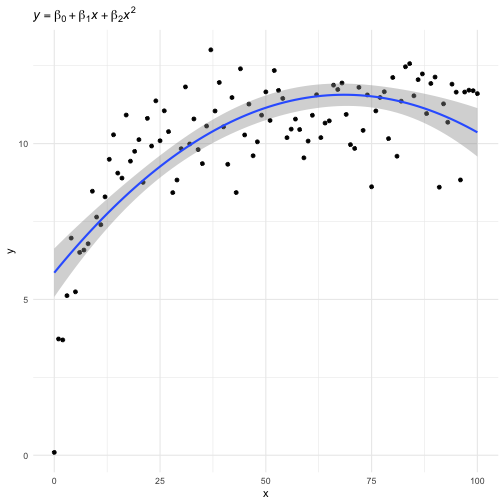
\includegraphics{gamm-presentation_files/figure-beamer/2-poly-1.pdf}

\end{frame}

\begin{frame}{LM with non-linear data}
\protect\hypertarget{lm-with-non-linear-data-5}{}

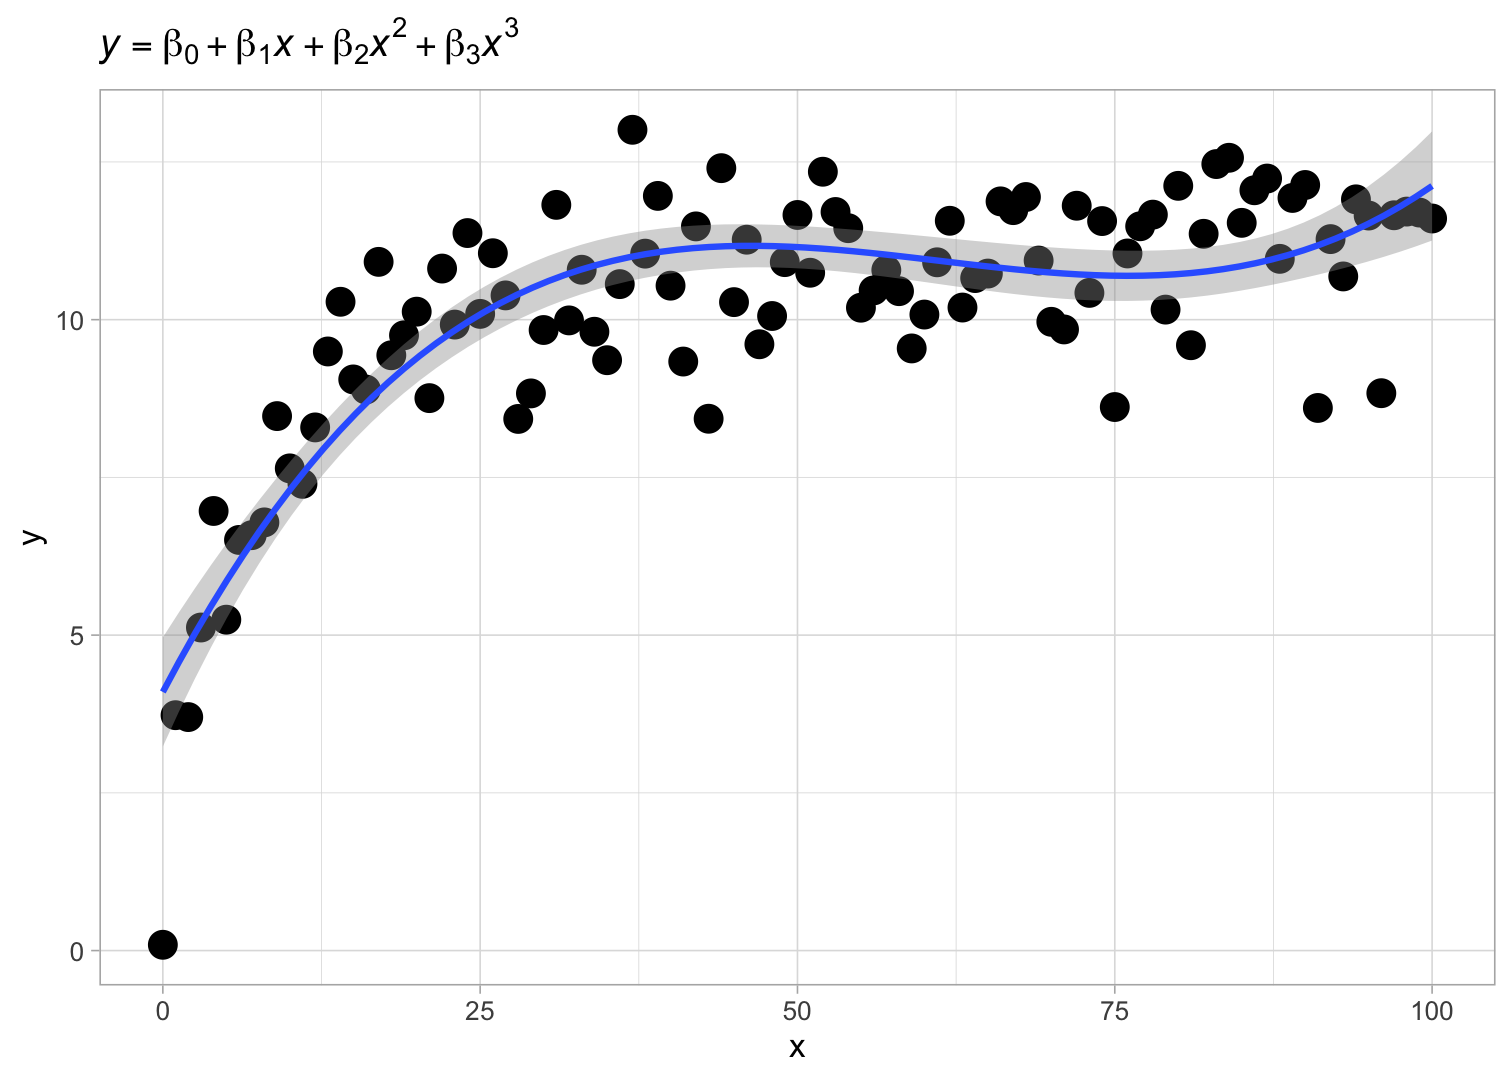
\includegraphics{gamm-presentation_files/figure-beamer/3-poly-1.pdf}

\end{frame}

\begin{frame}{LM with non-linear data}
\protect\hypertarget{lm-with-non-linear-data-6}{}

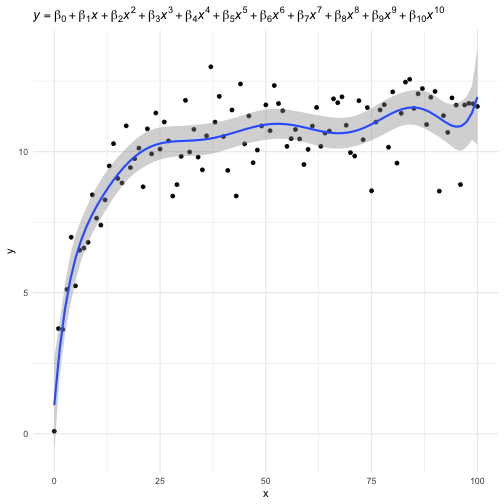
\includegraphics{gamm-presentation_files/figure-beamer/10-poly-1.pdf}

\end{frame}

\begin{frame}{LM with non-linear data}
\protect\hypertarget{lm-with-non-linear-data-7}{}

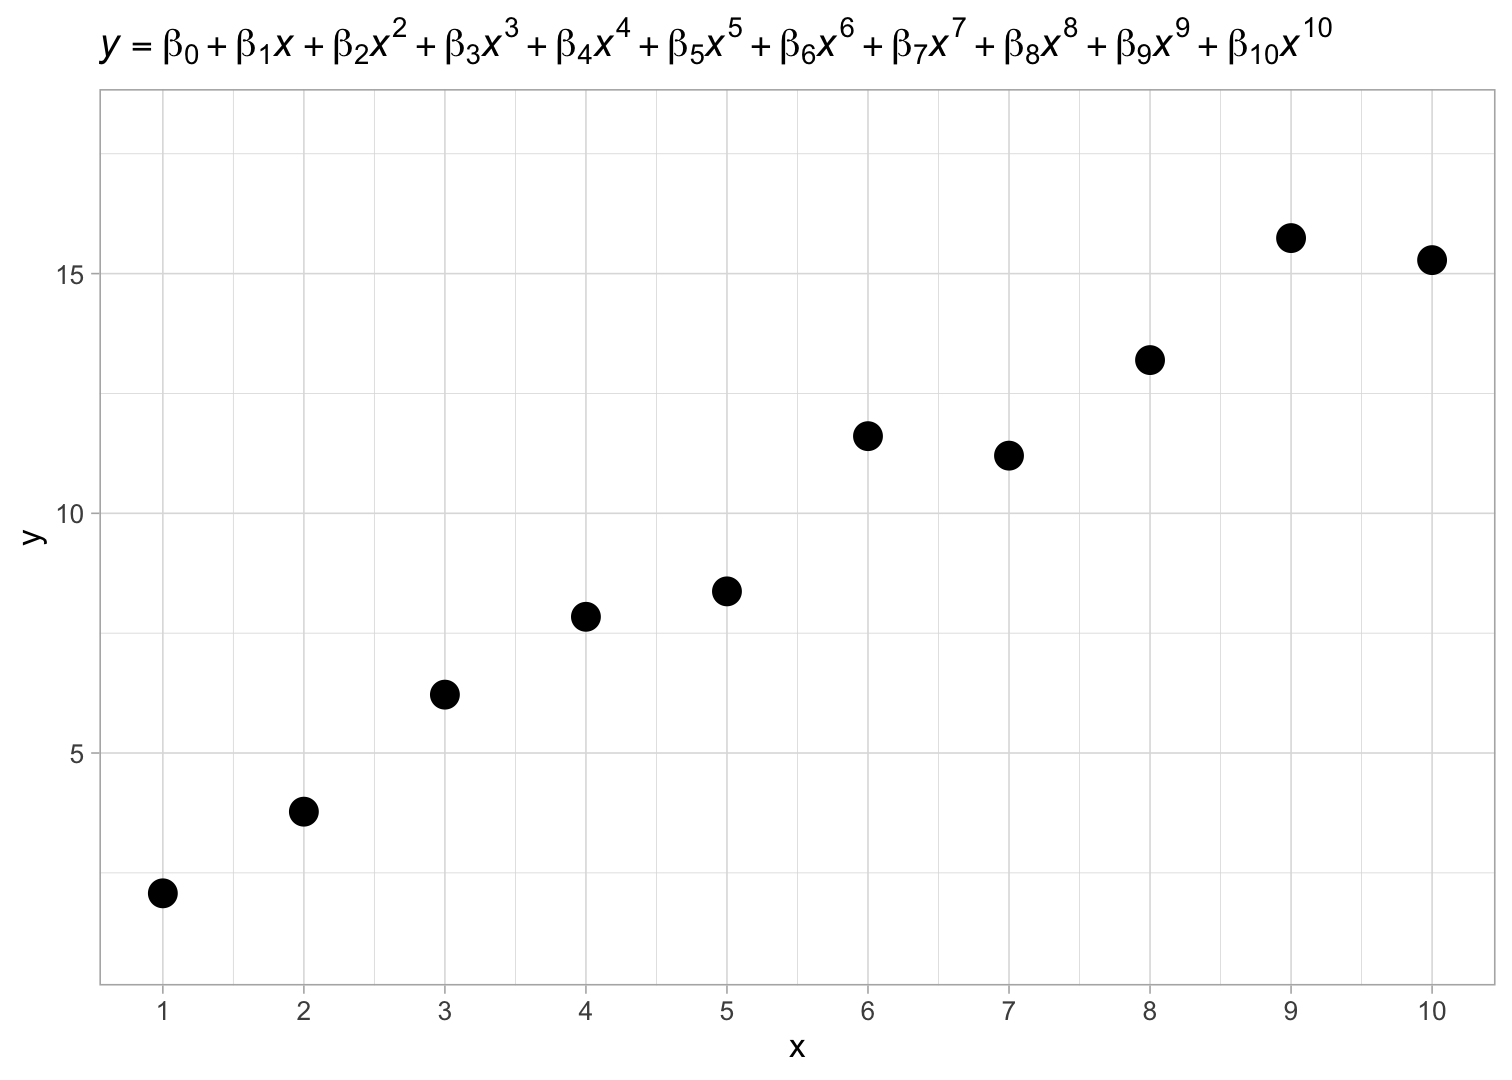
\includegraphics{gamm-presentation_files/figure-beamer/10-poly-2-1.pdf}

\end{frame}

\begin{frame}{Generalised additive models}
\protect\hypertarget{generalised-additive-models}{}

\begin{itemize}
\item
  \textbf{G}enrealised \textbf{A}dditive \textbf{M}odel\textbf{s}
\item
  \(y = f(x) + \epsilon\)

  \begin{itemize}
  \tightlist
  \item
    \(f(x)\) = `some function of \(x\)' (or \emph{smooth function})
  \end{itemize}
\end{itemize}

\end{frame}

\begin{frame}[fragile]{Smooth terms}
\protect\hypertarget{smooth-terms}{}

\begin{itemize}
\tightlist
\item
  LMs have \textbf{parametric terms}

  \begin{itemize}
  \tightlist
  \item
    \(\beta_nx_n\) (\texttt{x} in \texttt{R})
  \item
    linear effects
  \end{itemize}
\item
  GAMs add (non-parametric) \textbf{smooth terms} (or simply smooths,
  also smoothers)

  \begin{itemize}
  \tightlist
  \item
    \(f(x)\), \texttt{s(x)} in \texttt{R}
  \item
    non-linear effects
  \end{itemize}
\item
  \texttt{gam(y\ \textasciitilde{}\ s(x),\ data)}, `\(y\) as \emph{some}
  function of \(x\)'
\end{itemize}

\end{frame}

\begin{frame}{Smoothing splines, basis, basis functions}
\protect\hypertarget{smoothing-splines-basis-basis-functions}{}

\begin{itemize}
\tightlist
\item
  smooths in GAMs are \textbf{smoothing splines}

  \begin{itemize}
  \tightlist
  \item
    splines are defined piecewise with polynomials
  \item
    the piecewise combination of polynomials is called the
    \textbf{basis}
  \item
    the basis is composed of \textbf{basis functions} (the polynomials)
  \end{itemize}
\item
  there are \textbf{several kinds} of splines

  \begin{itemize}
  \tightlist
  \item
    each with their own basis functions
  \item
    thin plate regression splines
  \item
    cubic regression splines
  \end{itemize}
\end{itemize}

\end{frame}

\end{document}
